%---------------------------------------------------------------------
%
%                          Cap�tulo 1
%
%---------------------------------------------------------------------

\chapter{Introduccion}

\begin{FraseCelebre}
\begin{Frase}
     La atenci�n de los dem�s nos da el l�mite que hemos de poner a nuestras palabras. 
\end{Frase}
\begin{Fuente}
Noel Claras�
\end{Fuente}
\end{FraseCelebre}

\begin{resumen}
En este cap�tulo ...
\end{resumen}


%-------------------------------------------------------------------
\section{Escenario}
%-------------------------------------------------------------------
\label{cap1:sec:escenario}

Se pueden incluir acronimos  \gls{GPL} \footnote{y poner notas a pie de pagina sin problema a cualquier elemento}... la segunda vez que se use el acronimos ya no se muestra su significado, es decir \gls{GPL}.

Si quiero poner un link ha un parrafo en concreto del documento entonces pongo un una secci�n fantasma.

\phantomsection
\label{cap1:int:1}

Para incluir un link en la bibliografia hay que citarlo y decir por ejemplo ,v�ase \citep{CruiseControl}, ...

Para listar:

Se puede usar un enumerate:

\begin{enumerate}
    \item Algo
    \item mas cosas
    \item yepa
\end{enumerate}

O un itemize:

\begin{itemize}
    \item Algo
    \item mas cosas
    \item yepa
\end{itemize}

O cualquier combinaci�n de ambos:

\begin{itemize}
    \item Algo
    \item mas cosas
\begin{enumerate}
    \item Algo
    \item mas cosas
    \item yepa
\end{enumerate}
    \item yepa
\end{itemize}

Se pueden citar referencias muy facilmente, como por ejemplo la figura \ref{capitulos:fig:1/imagenprueba}.

Para incluir varias imagenes se puede usar:

\begin{figure}[h]   
    \begin{minipage}[t]{.45\textwidth}
        \begin{center}
            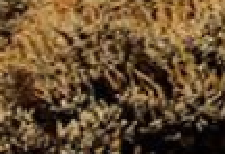
\epsfig{file=Imagenes/Vectorial/Capitulos/1/arbusto, scale=0.9} 
        \end{center}
    \end{minipage}
    \hfill
    \begin{minipage}[t]{.45\textwidth}
        \begin{center}
            
\epsfig{file=Imagenes/Vectorial/Capitulos/1/cielo, scale=0.9} 
        \end{center}
    \end{minipage}
    \caption{Comparativa de arbusto y cielo?}
    \label{capitulos:fig:1/imagenprueba}
    \hfill
\end{figure}



%-------------------------------------------------------------------
\section{�Que es otra secci�n?}
%-------------------------------------------------------------------
\label{cap1:sec:otra}



Sencillamente \textit{otra secci�n}. :) 

Como dijo pepito: 

\begin{quotation}
     blah blah blah
     llll

     11 22  3 4

\end{quotation}



\medskip

